%%%%%%%%%%%%%%%%%%%%%%%%%%%%%%%%%%%%%%%%%%%%%%%%%%%%%%%%%%%%%%%%%
%
% Project     : Bachelorarbeit
% Title       : Machbarkeitsanalyse für eine ressourcenorientierte Schnittstelle zur Verarbeitung grundlegender Probleme der Informatik
% File        : einleitung.tex Rev. 01
% Date        : 01.03.2015
% Author      : Raffael Santschi
%
%%%%%%%%%%%%%%%%%%%%%%%%%%%%%%%%%%%%%%%%%%%%%%%%%%%%%%%%%%%%%%%%%

\chapter{Einleitung}\label{chap.einleitung}
Die Einleitung dient dazu, wichtige Informationen zum Verständnis der Arbeit zu erläutern. Es werden die Komplexitätsklassen der Theoretischen Informatik und die verschiedenen Algorithmentypen erklärt.

\section{Komplexitätsklassen der Theoretischen Informatik}\label{cat_theo_inf}
In der Theoretischen Informatik wird zwischen verschiedenen Komplexitätsklassen unterschieden. In diesem Kapitel werden nur auf die Komplexitätsklassen NP, P, NP-schwer und NP-vollständig eingegangen, weitere Klassen wie zum Beispiel RP (Random Polynomial) oder ZPP (Zero-Error, Probabilistic, Polynomial) werden nicht erläutert, da sie nicht zum Verständnis der Arbeit notwendig sind. Die nachfolgenden Erklärungen sind aus \cite{hopcroft2011einfuehrung} und \cite{slides_p_np} abgeleitet.

\begin{figure}[h]
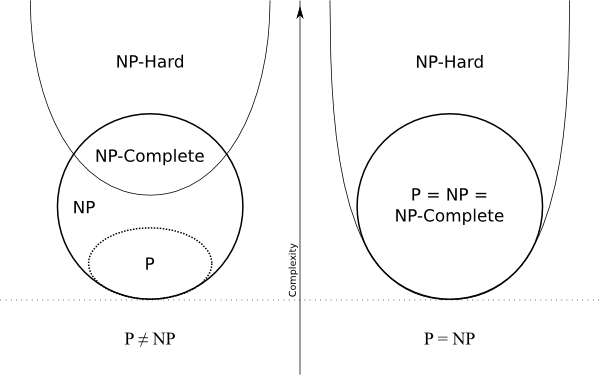
\includegraphics[scale=0.7]{images/einleitung/p_np_np-complete_np-hard.png}
\caption[Übersicht der Komplexitätsklassen ($P!=NP$ und $P=NP$)]{Übersicht der Komplexitätsklassen ($P \neq NP$ und $P=NP$) \cite{pic_p_np}}
\label{fig:complexity_overview}
\end{figure}

Die Abbildung \ref{fig:complexity_overview} zeigt die Aufteilung der verschiedenen Komplexitätsklassen für die beiden Fälle $P \neq NP$ und $P=NP$. Momentan wird davon ausgegangen, dass $P \neq NP$ ist und somit die linke Aufteilung stimmt. Keine der beiden Behauptungen konnte bis jetzt bewiesen werden. Der letzte Versuche $P \neq NP$ zu beweisen wurde von Vinay Deolalikar im Jahr 2010 unternommen \cite{p_neq_np_paper}. In diesem Versuch wurden jedoch zwei Fehler entdeckt (siehe \cite{p_neq_np_paper_blog}) und somit bleibt der Beweis weiter offen.

\subsection{NP}\label{np}
Falls die Korrektheit einer Lösung zu einem Problem in polynomialer Zeit überprüft werden kann, also ein Polynomialzeit-Verifizierer vorhanden ist, liegt das Problem in NP.

\subsection{P}\label{p_complet}
Probleme, welche in polynomialer Zeit lösbar sind, gehören zu der Klasse der P-vollständigen Probleme. In polynomialer Zeit lösbar heisst, dass die Laufzeitkomplexität in einem Polynom mit der Form $n^k$, wobei n die Eingabelänge und k eine Konstante ist, dargestellt werden kann.

\subsection{NP-schwer}\label{np_hard}
Probleme, welche nicht in polynomialer Zeit lösbar sind, das heisst eine Laufzeitkomplexität höher als polynomial haben, zum Beispiel $k^n$ (exponentiell) oder $n!$ (faktoriell), gehören zu den NP-schweren Problemen. Um zu beweisen, dass das Problem NP-schwer ist, wird versucht ein anderes bekanntes NP-schweres Problem auf dieses Problem zu reduzieren. Mit diesem Beweis wird gezeigt, dass das Problem mindestens so schwer wie das andere Problem ist.

\subsection{NP-vollständig}\label{np_complet}
Stephen Cook hat mit dem Beweis der NP-Vollständigkeit des SAT-Problems (siehe \cite{cook_complexity}), die Ausgangslage für den Beweise der NP-Vollständigkeit vieler weiteren Probleme bereit gestellt. Damit ein Problem als NP-vollständig gilt, müssen folgende zwei Punkte erfüllt sein:
\begin{itemize}
	\item Ein Polynomialzeit-Verifizierer für das Problem ist vorhanden.
	\item Ein anderes bekanntes NP-vollständiges Problem ist auf dieses Problem reduzierbar.
\end{itemize}

\section{Algorithmentypen}\label{algo_types}

\subsection{Backtracking Algorithmen}\label{backtracking_algos}
Beim Backtracking geht es darum, sich einer Lösung eines Problems schrittweise zu nähern. Bei jedem neuen Schritt wird geprüft, ob es noch eine gültige Lösung darstellt. Falls dies nicht der Fall ist, wird der letzte Schritt rückgängig gemacht und es wird ein anderer Weg eingeschlagen. In \cite{backtracking} wird dieses Verfahren an Hand des Damenproblems aufgezeigt.

\subsection{Greedy Algorithmen}\label{greedy_algos}
Greedy Algorithmen liefern oft eine schnelle Lösung, welche aber meist nicht optimal ist. Die Algorithmen entscheiden bei jedem Schritt, was die aktuell beste Möglichkeit ist. Da sie nicht alle Möglichkeiten betrachten, finden sie oft nur ein lokales Minimum bzw. Maximum. In \autoref{fig:greedy_algo} ist in grün der Weg des Greedy Algorithmus zu sehen. Der Algorithmus entscheidet sich für die 12 auf der zweiten Ebene, da diese in dem Moment als beste Lösung gilt. Mit dem violetten Pfad könnte jedoch einen viel höheren Wert erzielen werden.

\begin{figure}[h]
\centering 
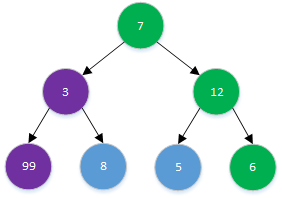
\includegraphics[scale=1]{images/einleitung/greedy_algo.png}
\caption[Suchablauf eines Greedy Algorithmus]{Suchablauf eines Greedy Algorithmus \cite{pic_greedy_algo}}
\label{fig:greedy_algo}
\end{figure}

\subsection{Evolutionäre Algorithmen}\label{ea_algos}
Evolutionäre Algorithmen nähern sich einer optimalen Lösung an. Sie basieren auf Kombinationen (Generationen) von Objekten und einer Fitnessfunktion zur Bewertung der einzelnen Generationen. Ein Ablauf eines Evolutionären Algorithmus sieht meist wie folgt aus:
\begin{enumerate}
	\item Initialisierung: Die erste Generation wird meist zufällig erzeugt
	\item Iteration durch folgende Schritte bis die Lösung den gewünschten Wert erreicht hat:
     	\begin{enumerate}
		\item Evaluation: Mit Hilfe der Fitnessfunktion wird die erstellte Generation bewertet
         		\item Selektion: Auswahl von Objekten (Individuen) für die Rekombination
         		\item Rekombination: Erstellen einer neuen Generation durch die Kombination der ausgewählten Individuen
         		\item Mutation: Veränderung der Eigenschaften (Gene) der Nachfahren
      	\end{enumerate}
\end{enumerate}
Die Mutation und Rekombination kann positive, negative oder neutrale Eigenschaften haben. Wie in der Natur überlebt der Stärkste und somit wird die Lösung immer besser.
